%% LyX 2.3.3 created this file.  For more info, see http://www.lyx.org/.
%% Do not edit unless you really know what you are doing.
\documentclass[oneside,english,a4paper,11pt,final,DIV13,BCOR20mm,openbib,openright,onecolumn,pagesize,pointlessnumbers,bibtotoc,liststotoc,idxtotoc,bigheadings,titlepage,tocindent,intoc,pdftex,utf8]{scrbook}
\usepackage[T1]{fontenc}
\usepackage[utf8]{inputenc}
\setcounter{secnumdepth}{3}
\setcounter{tocdepth}{3}

\makeatletter
%%%%%%%%%%%%%%%%%%%%%%%%%%%%%% User specified LaTeX commands.
\NeedsTeXFormat{LaTeX2e}
%\documentclass[a4paper,11pt,final,DIV13,BCOR20mm,openbib,twoside, openright,onecolumn,pagesize,pointlessnumbers,bibtotoc,liststotoc,idxtotoc,
%	bigheadings,titlepage,tocindent,intoc,pdftex]{scrbook}
\usepackage{emptypage}
\usepackage[ngerman]{babel}
%\usepackage[utf8]{inputenc}
%\usepackage[ansinew]{inputenc}
%\usepackage{blindtext}
%\usepackage[T1]{fontenc}
%\usepackage{bibgerm}
%\usepackage{lmodern}
%\usepackage{url}
%\usepackage{microtype}
%\usepackage{tabularx}
%\usepackage{xcolor}
%\usepackage[pdftex]{graphicx}
%\usepackage{amsmath}

%\usepackage{amsthm}
%\usepackage{amssymb}
%\usepackage{pdfpages}
%%\usepackage{subfig}
%\usepackage{subfigure}
%\usepackage{rotating}
%\usepackage{nextpage}
%\usepackage[numbers,sort&compress]{natbib}
%\usepackage{float}
%\usepackage{algorithm}
%\usepackage{algorithmicx}
\makeatletter
%\renewcommand*{\ALG@name}{Algorithmus}
\makeatother
\usepackage{algpseudocode}
\algtext*{EndIf}
\usepackage{lscape}
\usepackage[absolute]{textpos}
\setlength{\TPHorizModule}{1mm}
\setlength{\TPVertModule}{\TPHorizModule}
\textblockorigin{0mm}{0mm}
\usepackage{parskip}
\begingroup
\expandafter\expandafter\expandafter\endgroup
\expandafter\ifx\csname chapterformat\endcsname\relax\else
    \renewcommand*{\chapterformat}{
        \llap{
            \chapappifchapterprefix{\ }\thechapter\autodot\enskip
        }
    }
\fi
\renewcommand*{\othersectionlevelsformat}[1]{
    \llap{
        \csname the#1\endcsname\autodot\enskip
    }
}
\setlength{\unitlength}{1mm}
\newlength{\grafikdim}
\usepackage{listings}
\usepackage{color}
\renewcommand{\ttdefault}{pcr}
\renewcommand{\lstlistingname}{Codeausschnitt}
%JAVA
\definecolor{darkblue}{rgb}{0,0,.6}
\definecolor{darkred}{rgb}{.6,0,0}
\definecolor{forestgreen}{RGB}{34,139,34}
\definecolor{lgreen}{RGB}{50,201,50}
\definecolor{red}{rgb}{.98,0,0}
\definecolor{lbrown}{rgb}{0.54,0.27,0.01}
\definecolor{purple}{rgb}{0.5,0,0.33}
%XML
\definecolor{forestgreen}{RGB}{34,139,34}
\definecolor{orangered}{RGB}{239,134,64}
\definecolor{gray}{rgb}{0.4,0.4,0.4}
\lstdefinestyle{JAVA}{
  language=JAVA,
  captionpos=b, % Beschriftung ist unterhalb
  basicstyle=\ttfamily\small, % Schriftart&Größe
  commentstyle=\itshape\color{forestgreen},
  keywordstyle=\bfseries\color{purple},
  stringstyle=\color{blue},
  showspaces=false,
  showtabs=false,
  columns=fixed,
  frame=none,
  breaklines=true,
  showstringspaces=false,
  frame=tb,
	moredelim=[is][\itshape]{__}{__},
	moredelim=[is][\textcolor{lbrown}]{~~}{~~},
	moredelim=[is][\textcolor{blue}]{++}{++},
	moredelim=[is][\itshape\bfseries\textcolor{darkblue}]{**}{**}
}
\lstdefinestyle{JAVA_LN}{
  language=JAVA,
  captionpos=b, % Beschriftung ist unterhalb
  basicstyle=\ttfamily\small, % Schriftart&Größe
  commentstyle=\itshape\color{forestgreen},
  keywordstyle=\bfseries\color{purple},
  stringstyle=\color{blue},
  showspaces=false,
  showtabs=false,
  columns=fixed,
  frame=none,
  numbers=left, % Zeilennummern links vom Code
  numberstyle=\tiny, % kleine Zeilennummern
  numbersep=5pt,
  breaklines=true,
  showstringspaces=false,
  xleftmargin=0.7cm,
  frame=tb,
	moredelim=[is][\itshape]{__}{__},
	moredelim=[is][\textcolor{lbrown}]{~~}{~~},
	moredelim=[is][\textcolor{blue}]{++}{++},
	moredelim=[is][\itshape\bfseries\textcolor{darkblue}]{**}{**}
}
\lstdefinestyle{XML} {
    language=XML,
    captionpos=b, % Beschriftung ist unterhalb
    basicstyle=\ttfamily\small,
    columns=fullflexible,
    commentstyle=\color{gray}\upshape,
    %keywordstyle=\color{orangered},
    stringstyle=\ttfamily\color{black}\normalfont,
    tagstyle=\color{darkblue}\bfseries,
    extendedchars=true, 
    breaklines=true,
    breakatwhitespace=true,
    emph={},
    emphstyle=\color{red},
    morestring=[b]",
    morecomment=[s]{<?}{?>},
    morecomment=[s][\color{forestgreen}]{<!--}{-->},
    morekeywords={attribute,xmlns,version,type,release},
    frame=tb
}
\lstdefinestyle{XML_LN} {
    language=XML,
    captionpos=b, % Beschriftung ist unterhalb
    basicstyle=\ttfamily\small,
    columns=fullflexible,
    commentstyle=\color{gray}\upshape,
    %keywordstyle=\color{orangered},
    stringstyle=\ttfamily\color{black}\normalfont,
    tagstyle=\color{darkblue}\bfseries,
    numbers=left, % Zeilennummern links vom Code
  	numberstyle=\tiny, % kleine Zeilennummern
  	numbersep=5pt,
    extendedchars=true, 
    breaklines=true,
    breakatwhitespace=true,
    emph={},
    emphstyle=\color{red},
    morestring=[b]",
    morecomment=[s]{<?}{?>},
    morecomment=[s][\color{forestgreen}]{<!--}{-->},
    morekeywords={attribute,xmlns,version,type,release},
    frame=tb
}
\lstdefinestyle{JSON} {
    captionpos=b, % Beschriftung ist unterhalb
    basicstyle=\small,
    columns=fullflexible,
    extendedchars=true, 
    breaklines=true,
    breakatwhitespace=true,
    string=[s]{"}{"},
    stringstyle=\color{darkblue}\ttfamily\bfseries,
    comment=[l]{:},
    commentstyle=\color{black}\ttfamily,
		frame=tb
}
\usepackage[simplified]{pgf-umlcd}
\renewcommand{\umltextcolor}{black}
\renewcommand{\umlfillcolor}{white}
\renewcommand{\umldrawcolor}{black}
\setcounter{secnumdepth}{2}
\setcounter{tocdepth}{2}
\setlength{\parskip}{\medskipamount}
\setlength{\parindent}{0pt}
\usepackage{soul}
\makeindex
\usepackage{nomencl}
\providecommand{\printnomenclature}{\printglossary}
\providecommand{\makenomenclature}{\makeglossary}
\makenomenclature
\AfterFile{t1lmss.fd}{
  \DeclareFontShape{T1}{lmss}{b}{n}
  {<->ssub*lmss/bx/n}{}
}
\usepackage{textcomp}
% Fehlerhaft bei mir. Teilweise werden Buchstaben in der PDF View in Eclipse
% nicht angezeigt.
%\usepackage[charter]{mathdesign}
\usepackage{footmisc}
\DeclareSymbolFont{cmsy}{OMS}{cmsy}{m}{n}
\DeclareSymbolFontAlphabet{\mathcal}{cmsy}
\usepackage{fancyhdr}
\usepackage{setspace}
\PassOptionsToPackage{hyphens}{url}\usepackage{hyperref}
\onehalfspacing
\pagestyle{headings}
\newcommand*{\ORIGchapterheadendvskip}{}
\let\ORIGchapterheadendvskip=\chapterheadendvskip
\renewcommand*{\chapterheadendvskip}{
    {
        \setlength{\parskip}{0pt}
        \noindent\rule{.3\textwidth}{3pt}\rule[2.5pt]{.7\linewidth}{.5pt}\par
    }
    \vskip1.2em
}
\makeatletter
\providecommand{\toclevel@lstlisting}{0}
\makeatother
\addtokomafont{caption}{\small}
\setkomafont{captionlabel}{\sffamily\bfseries}
\setcapindent{1em}
\renewcommand \theparagraph {(\arabic{paragraph})}
\pagestyle{fancy}
\usepackage{calc}
\renewcommand{\chaptermark}[1]{\markboth{#1}{}}
\renewcommand{\sectionmark}[1]{\markright{\thesection\ #1}}
\fancyhf{}
\fancyfoot[RO]{\rightmark\quad{\bfseries\thepage}}
\fancyfoot[LE]{{\bfseries\thepage}\quad\leftmark}
\renewcommand{\headrulewidth}{0pt}
\fancypagestyle{plain}{
  \fancyhf{}
  \fancyfoot[RO]{{\bfseries\thepage}}
  \fancyfoot[LE]{{\bfseries\thepage}}
  \renewcommand{\headrulewidth}{0pt}
}
\usepackage{booktabs}
\usepackage{pifont}
\setlength{\nomlabelwidth}{.20\hsize}
\renewcommand{\nomlabel}[1]{#1 \dotfill}
\hyphenation{name-space}
\usepackage{array}
\usepackage{bigstrut}
\graphicspath{{../img/}}
\newcolumntype{Y}{>{\centering\arraybackslash}X}
\usepackage{bibgerm}
\usepackage{graphicx}

\makeatother

\begin{document}
\pagenumbering{gobble}\begin{titlepage}
\newcommand{\Titel}[2][\textwidth]{\renewcommand{\baselinestretch}{1.0}\hfil
            \parbox{#1}{\huge\bfseries\centering #2}\hfil\par}
\renewcommand{\subtitle}[2][\textwidth]{\renewcommand{\baselinestretch}{1.0}\hfil
            \parbox{#1}{\LARGE\centering\mbox{}\llap{--~}#2\rlap{~--}}\hfil\par}
\newcommand{\addLine}[2][\textwidth]{\renewcommand{\baselinestretch}{1.0}\hfil
            \parbox{#1}{\large\centering #2}\hfil\par}


\begin{textblock}{40}(30,27)
 
\includegraphics[scale=0.7]{img/unilogo.pdf}
\end{textblock}

\begin{textblock}{40}(120,15)
 
\includegraphics[scale=0.07]{img/vs-color.pdf}
\end{textblock}

\addLine{}
\vspace{0.2\textheight}

\Titel{Automatisiertes Aufsetzen eines Kubernetes-Clusters auf Raspberry Pis mithilfe von Ansible-Playbooks}
%\vspace{0.09\textheight}

\newcommand*{\student}{KL}
\newcommand*{\matrikelnummer}{-}
\newcommand*{\betreuerA}{RH}
\newcommand*{\betreuerB}{HB}
\IfFileExists{titel-info}{\input{titel-info}}

\vspace{0.05\textheight}
\addLine{Seminararbeit von}
\addLine{\LARGE \student}
\addLine{Matrikelnummer:}
\addLine{\LARGE \matrikelnummer}
\addLine{Vorgelegt im Fachgebiet}
\addLine{\LARGE Verteilte Systeme}
\vspace{0.05\textheight} 
\addLine{
  \begin{tabbing}
   Betreuer: \quad ~\= \betreuerA\\
   Betreuer: \quad ~\= \betreuerB
  \end{tabbing}
}
\vspace{0.05\textheight} 
\addLine{\today}
\vspace{0.05\textheight} 
\addLine{Universität Kassel}
\addLine{Fachbereich Elektrotechnik und Informatik}
\addLine{Wintersemester 2019/2020}
\end{titlepage}

%\cleartooddpage[\thispagestyle{empty}]
%\newpage
%\cleartooddpage[\thispagestyle{empty}]
%\thispagestyle{empty}

%\thispagestyle{empty}
%\cleardoublepage



\cleardoublepage{}

\chapter*{Erklärung}

\vfill

Hiermit versichere ich, dass ich die vorliegende Seminararbeit selbstständig
verfasst und nur die angegebenen Hilfsmittel und Quellen benutzt habe. Alle
Stellen, die wörtlich oder sinngemäß aus veröffentlichten oder
unveröffentlichten Schriften entnommen sind, habe ich als solche kenntlich
gemacht. Diese Seminararbeit wurde bis jetzt noch nicht veröffentlicht und
wurde bisher noch in keinem anderen Prüfungsamt vorgelegt.
\newline
\newline

\qquad Kassel, den \today \hfill
\rule{0.45\textwidth}{0.4pt}

\vfill 


\cleardoublepage{}

\addtocontents{toc}{\protect\enlargethispage{2\normalbaselineskip}}

\tableofcontents{}

\listoffigures

\thispagestyle{empty}
%\cleartooddpage[\thispagestyle{empty}]
\pagenumbering{arabic}
\setcounter{page}{1}

%
\chapter{Einleitung}

\cite{Misc1,book1}

\section{Zielsetzung}

\section{Inhaltlicher Aufbau der Arbeit}

%
\chapter{Verwandte Arbeiten}

\chapter{Grundlagen}

%
\chapter{Entwurf}

%
\chapter{Implementierung}

%
\chapter{Evaluierung}

%
\chapter{Fazit}


\chapter{Einleitung}\label{ch:einleitung}

Kubernetes ist eine moderne Technologie, die skalierbare Applikationen ermöglicht.
Sie beruht auf dem Prinzip, mehrere Rechner miteinander zu vernetzen und ihre gesamten Ressourcen effizient zu nutzen.
In Produktivumgebungen werden dazu leistungsstarke Maschinen oder Cloud-Instanzen eingesetzt.
% TODO finanz nicht so wichtig, vorteile von lokal hervorheben, warum überhaupt cluster? fork computing, mobile edge computing
Im Entwicklungsbetrieb kann es jedoch von Vorteil sein, aus finanziellen Gründen auf die Leistungsfähigkeit und die gute Anbindung eines Rechenzentrums zu verzichten und stattdessen auf lokal betriebene Systeme zu setzen.
% TODO raspi verlinken
Eine besonders günstige Option stellen hierbei Einplatinencomputer wie der Raspberry Pi dar.

Es sind viele Schritte nötig, um einen Kubernetes-Cluster einzurichten und je mehr Nodes eingerichtet werden sollen, umso häufiger müssen die immer gleichen Schritte durchgeführt werden.
Mithilfe des Automatisierungs-Werkzeugs Ansible können diese Aufwände automatisiert und somit vereinfacht und beschleunigt werden.
Nachdem mit wenigen Handgriffen das Standardbetriebssystem Raspbian installiert wurde, werden alle weiteren Schritte von Ansible-Playbooks automatisch erledigt.

In dieser Seminararbeit werden zunächst die verwendeten Technologien, Kubernetes und Ansible, kurz vorgestellt (Kapitel~\ref{ch:technologien}).
Anschließend wird die Vorgehensweise zum Aufsetzen eines Clusters mithilfe der Playbooks übersichtlich zusammengefasst (Kapitel~\ref{ch:anwendung}).
Danach erfolgt eine ausführliche Erläuterung der Funktionsweise der Playbooks (Kapitel~\ref{ch:umsetzung}).
Zuletzt werden mögliche Alternativen zu den eingesetzten Technologien vorgestellt (Kapitel~\ref{ch:alternativen}) und ein Ausblick auf mögliche Weiterentwicklungen gegeben (Kapitel~\ref{ch:zusammenfassung}).
\chapter{Anwendung}\label{ch:anwendung}

Um mithilfe der Playbooks aus diesem Projekt einen Kubernetes-Cluster einzurichten, müssen zunächst die WiFi-Infrastruktur und die Raspberry Pis vorbereitet werden.
Dazu werden die SD-Karten einzeln mit Raspbian beschrieben und mit dem Playbook \texttt{local-""raspbian.yaml} für den Headless-Betrieb\footnote{Betrieb ohne Bildschirm} konfiguriert, mit Strom versorgt und gestartet.
Sobald alle Raspberry Pis online sind, wird Kubernetes mit dem Playbook \texttt{kubernetes.yaml} aufgesetzt.

\begin{figure}[h]
    % https://www.draw.io/?title=ansible-kubernetes-anwendung#R7Vlbd6IwEP41PuoBgoqPK73stt2trdt2%2B7QnSoTUQNgQqu6v3wBBwFhLd721Z33wkEkml2%2Fmm5lAA9j%2B%2FJzB0PtKHUQahubMG%2BCkYRidblf8J4JFJgAdLRO4DDuZSC8EQ%2FwbSWE%2BLMYOiioDOaWE47AqHNMgQGNekUHG6Kw6bEJJddUQukgRDMeQqNIH7HAvk1pGt5B%2FRtj18pX1Ti%2Fr8WE%2BWJ4k8qBDZyUROG0Am1HKsyd%2FbiOSYJfj8vBl8UCupp3zi5voF7zrX37%2Fdt%2FMJjt7i8ryCAwF%2FK%2Bnvn6M4N2nm%2Blvt%2Bs%2F65bZu7%2F50ZRnfYYklnjJs%2FJFDiByBJ6ySRn3qEsDSE4LaZ%2FROHBQsowmWsWYK0pDIdSF8AlxvpDOAWNOhcjjPpG9Nc8ncYhozMZow6GAdDPIXMQ3jLOycckBS74i0TtH1EecLcQAhgjk%2BLnqUFD6pbscV2AvHiT8bzAFUExxC6NwhGGQaAYRh4RgJCBSLFTgn4A58zBHwxCmEM0Ep%2F8F62fEOJpvRCfvNSVNZJzoyeasIJ2exwSvRLhcbft4gkO4Mppj%2FiNRb7Vl67HUczKXM6eNRd4IxHlLSknzsdxXqKWtXG%2FLtLFq0gYYR8UbS%2BHNgMDFiNJpw%2BgQcZD%2BiIknl6eIZZIJFYiJZAIlIJ1fcRLF%2B7bASHBMdH1Ds0KcqxMq8kqTLWmZTSZ2nc1XXaNYFcbRpGGDRt%2F23g199XZN%2FrZ3xV%2B995%2B%2Fb%2BKvXjfvgaPir64mvuFJ8xIKz00Tn%2Fi7wkE8bw7sZNM4IMh9LywCe0yC5On69IthfO1fxfZZ%2FMSjW%2FehaX7I%2Bs5QHX18ez%2B%2BnNoXZ5%2FC7sQ2m2LvI1kQH4uj59ve4OhpxYdYuqkBfnfuvrwqHSxpgI6CcYCwCt8%2BM0kpjxRZ5ZVMolfySJFW9pNJgFkzk%2BjHlUqAWgs%2BwUPaXv8b22vvw%2Fage1y2V1PdEAdOshQhKI2nUfI6ComLtIhv4mRnalD1qD%2BKo9cDKiTYDcTzWGAurgu7i7BAWynLawZYa1cFhZrDPkJBsXVXlqoDitOLprRm29JamviZJjBBx8qj5yJPii3NsNpd3cz%2BV6bPCClnXLHicov%2FwJ%2BuYtmd3aOnsShyAsRR9KHu0GZ7pRxq768aWktWXTHp8ZP1ADXHerLqRtWaq1bKoso2%2BLjWduqt%2BPhtVw60my5kr9cW5qFqi03bXn01X76oZVXFkQam1SqidmTaxnuJIbsdoMueb7oXJ95dYI1Ddr0GUdW7CcFhhKoIRR4Mk34UOEMOedI7wYTYlFCWqgEt%2FSVDOaNTtK7nBfjqIv8izG1r5e2PijJYAzLYFcg1wn8GUv5h1FgPtj93k0%2FDrQmhs7En%2FLyVevtP4wWP3hW%2BvX3BK5rFZ90soBffxsHpHw%3D%3D
    \centering
    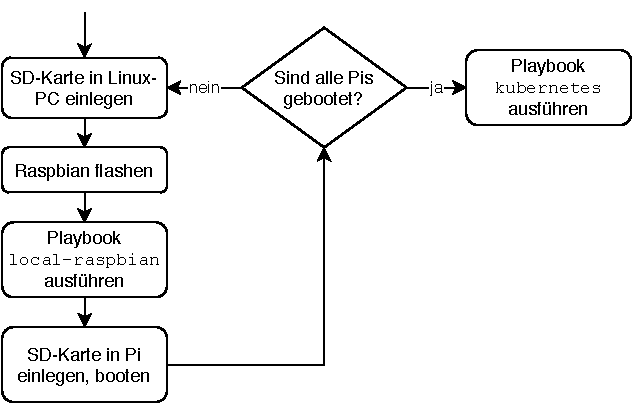
\includegraphics[width=\textwidth]{img/anwendung.pdf}
    \caption{Ablaufdiagramm zur Einrichtung eines Clusters}
\end{figure}

\section{Vorbereitung}\label{sec:vorbereitung}
Zum erfolgreichen Ausführen dieser Anleitung müssen folgende Voraussetzungen erfüllt sein:

\textbf{Raspberry Pis} in beliebiger Anzahl und ebenso viele Speicherkarten und Netzteile stehen bereit.

\textbf{Ein Linux-Rechner} steht bereit, um die Speicherkarten zu beschreiben und die Ansible-Playbooks auszuführen. Dafür sind Balena Etcher\footnote{\url{https://www.balena.io/etcher/} -- \today} und Ansible\footnote{\url{https://www.ansible.com/} -- \today} installiert, das Git-Repository zu diesem Projekt mit den Verzeichnissen \texttt{inventory} und \texttt{playbook} ist lokal verfügbar und auf dem aktuellen Stand und ein Image von Raspbian Lite\footnote{\url{https://downloads.raspberrypi.org} -- \today} ist heruntergeladen.
% https://downloads.raspberrypi.org/raspbian_lite/images/raspbian_lite-2020-02-14/2020-02-13-raspbian-buster-lite.zip

\textbf{Ein Terminal} mit \texttt{playbook} als Arbeitsverzeichnis ist geöffnet.

\textbf{Ein WiFi-Access Point} mit Internetzugriff ist in Betrieb. Seine Einstellungen (IP, SSID, WPA2-Key) entsprechen den Angaben in den Dateien \texttt{inventory/""group\_vars/""all.yaml} und \texttt{playbook/""local-""raspbian.yaml}. Der zuvor erwähnte Linux-Rechner ist mit dem Access Point verbunden.

\textbf{Die Inventory-Datei} \texttt{inventory/""k8s-cluster.yaml} bildet den derzeitigen Cluster ab -- enthält also keine Einträge unter \texttt{hosts}, falls ein neuer Cluster eingerichtet werden soll:

\begin{lstlisting}[language=yaml, caption=Leere Inventory-Datei]
nodes:
  hosts:
\end{lstlisting}

\textbf{Ein SSH-Schlüsselpaar} ist generiert. Der private Schlüssel ist auf dem Linux-PC unter \texttt{\$HOME/"".ssh} hinterlegt und der öffentliche Schlüssel im Playbook \texttt{local-""raspbian"".yaml} in dem Array \texttt{sshKeys}.

\section{Raspbian installieren und Cluster einrichten}\label{sec:raspbian-installieren}
Die folgenden Schritte müssen für jeden Raspberry Pi einzeln durchgeführt werden.

\begin{enumerate}
    \item Speicherkarte in den Linux-Rechner einlegen.
    \item Raspbian-Image mit Balena Etcher auf der Speicherkarte installieren.
    \item Raspbian-Playbook ausführen:
        \begin{lstlisting}
sudo ansible-playbook -i ../inventory/k8s-cluster.yaml local-raspbian.yaml
\end{lstlisting}
    \item Speicherkarte in den Raspberry Pi einsetzen und starten.
\end{enumerate}

Wenn alle Raspberry Pis gestartet sind, wird die Installation mit dem Kubernetes-Playbook fortgesetzt:

\begin{lstlisting}
ansible-playbook -i ../inventory/k8s-cluster.yaml kubernetes.yaml
\end{lstlisting}
\caption{CLI-Befehl zur Ausführung des Raspbian-Playbooks}

Der Kubernetes-Cluster ist anschließend einsatzbereit.

\section{Weitere Nodes hinzufügen}\label{sec:weitere-nodes-hinzufügen}

Sollen zu einem fertigen Cluster weitere Nodes hinzugefügt werden, kann auch dafür diese Anleitung ab Abschnitt~\ref{sec:vorbereitung} verwendet werden.
Die Inventory-Datei darf dann nicht leer sein, sondern muss die bereits vorhandenen Nodes enthalten.

\chapter{Technologien}\label{ch:technologien}

In diesem Kapitel werden die eingesetzten Technologien vorgestellt.
Nacheinander werden die Automatisierungssoftware Ansible, die Virtualisierungssoftware Docker sowie die Orchestrierungssoftware Kubernetes eingeführt.
Im Kapitel~\ref{ch:umsetzung} wird anschließend beschrieben, wie sich ein Kubernetes-Cluster, der Docker-Container verteilt und redundant laufen lassen und skalieren kann, mithilfe von Ansible automatisiert aufsetzen lässt.

\section{Ansible}\label{sec:ansible}

Ansible ist eine Software zur Automation von IT-Prozessen und Konfigurationsverwaltung.

Ein mit Ansible ausgerüsteter Steuer-Computer verbindet sich per SSH oder über andere Remote-Protokolle mit anderen Computern und führt auf ihnen Befehle aus, die einen Zielzustand herstellen sollen.
Dieser Zielzustand wird in sogenannten \emph{Playbooks} definiert.
Dabei handelt es sich um Textdateien im YAML-Format.

Sie bestehen im Wesentlichen aus einer Folge von \emph{Tasks}, die auf vordefinierte Ansible-Module zurückgreifen oder explizit auszuführende Terminal-Befehle enthalten.
\emph{Inventory}-Dateien werden angelegt, um die zu verwaltende Infrastruktur zu beschreiben.
Dafür werden die zu steuernden Hosts aufgelistet und gegebenenfalls kategorisiert.
Playbooks können bei der Ausführung dann auf einzelne Hosts oder bestimmte Gruppen beschränkt werden.

Auf den Remote-Hosts ist außer einem aktiven SSH-Dienst und einem Python-Interpreter keine weitere Software erforderlich.
Insbesondere wird kein Ansible-eigener Agent oder Ähnliches benötigt, sodass der Aufwand zur Vorbereitung der Hosts für die Verwaltung mit Ansible gering ausfällt.

\section{Docker}\label{sec:docker}

Docker ermöglicht Virtualisierung von Software.

In einem \emph{Docker-Container} laufen Programme isoliert von den Ressourcen das Host-Systems.
Neben Sicherheitsaspekten trägt dies auch zu einer erhöhten Portabilität von Anwendungen bei.
Mehrere Dienste, ihre Konfiguration und Abhängigkeiten zu installierten Bibliotheken lassen sich bündeln und auf unterschiedlichen Host-Systemen reproduzierbar ausführen.
Ein Container entsteht durch die Instanziierung eines \emph{Docker-Images}.
Diese sind vergleichbar mit einer Bauanleitung für das System, das im Container laufen soll.

In öffentlichen Verzeichnissen wie Docker Hub stehen zahlreiche Images zur Verfügung, die als Grundlage für eigene, darauf aufbauende Images dienen.

\section{Kubernetes}\label{sec:kubernetes}

Kubernetes ermöglicht den ausfallsicheren Betrieb virtualisierter Anwendungen mit automatischer Skalierung.

Ein Kubernetes-Cluster besteht aus mehreren, vernetzten Rechnern (\emph{Nodes}), die jeweils mit Docker oder einer vergleichbaren Virtualisierungssoftware ausgestattet sind.
Neben einer Vielzahl an \emph{Worker-Nodes} hat der Cluster eine Kontrollebene, die auf einem \emph{Master-Node} läuft.

Diese Kontrollebene verwaltet die Worker-Nodes und alle darauf laufenden Dienste.
Sie kann Dienste mit einer vorgegebenen Anzahl an Instanzen auf die Worker-Nodes verteilen, die Ausführung überwachen und bei Bedarf (beispielsweise bei einem Hardwareausfall) automatisch neue Instanzen hochfahren.
Anfragen an die im Cluster laufenden Dienste werden ebenfalls von der Kontrollebene entgegengenommen und die Last gleichmäßig auf laufende Instanzen verteilt.

\chapter{Umsetzung}\label{ch:umsetzung}

Um eine maximale Automatisierung zu erreichen, werden so viele Arbeitsschritte wie möglich von Ansible-Playbooks übernommen.
Zwei relevante Playbooks übernehmen unterschiedliche Aufgaben und unterscheiden sich grundsätzlich in ihrer Funktionsweise:
Bevor mit \texttt{kubernetes.yaml} die eigentliche Einrichtung des Clusters per gleichzeitigem Zugriff auf die Raspberry Pis via SSH vorgenommen werden kann, müssen die Systeme mit \texttt{local-raspbian.yaml} zunächst auf den Headless-Betrieb vorbereitet werden.
Dies geschieht ausschließlich über lokale Aktionen mit direktem Zugriff auf das Dateisystem der SD-Karten vom Linux-Rechner aus.

\section{Raspbian einrichten}\label{sec:raspbian-einrichten}

Das originäre Raspbian kann sich mangels Zugangsdaten (SSID und WPA-Key) nicht mit dem WiFi verbinden.
Gewöhnlicherweise werden diese Daten nach dem ersten Systemstart per Hand eingegeben.
Da dieser Schritt auf jedem einzelnen Raspberry Pi durchgeführt werden müsste und das Anschließen eines Monitors und einer Tastatur erfordern würde, entsteht dabei ein Aufwand, der sich durch Automatisierung vermeiden lässt.

Die WiFi-Konfiguration kann alternativ vorgenommen werden, indem die entsprechende Konfigurationsdatei von Raspbian direkt auf der SD-Karte angepasst wird.
Da die SD-Karte ohnehin zunächst einmal an einem separaten PC mit einem System-Image beschrieben werden muss, bietet sich dieser Zeitpunkt an, um weitere Konfigurationen vorzunehmen.
Neben der Einrichtung des kabellosen Netzwerks können hier auch weitere Schritte erledigt werden, die in den folgenden Unterkapiteln näher beschrieben werden.
Die Reihenfolge kann dabei - mit Ausnahme des Mountens und Unmountens der Partitionen - beliebig geändert werden.

Für diese Schritte gibt es das Playbook \texttt{local-""raspbian"".yaml}.
Da der Rasperry Pi zum Ausführungszeitpunkt dieses Playbooks nicht läuft, werden sämtliche enthaltenen Tasks auf dem Ansible-Host ausgeführt, nicht auf Remote-Hosts.
Alle Aktionen erfolgen mittels direktem Zugriff auf das Dateisystem, anstatt ein laufendes System anzusprechen.
Dadurch beschränken sich die nutzbaren Ansible-Module auf jene, die das Dateisystem betreffen.

\subsection{Partitionen mounten}\label{subsec:partitionen-mounten}

Ein Raspbian-System besteht aus zwei Partitionen: eine Hauptpartition (\texttt{rootfs}) und eine Boot-Partition, die einen Zugriff auf häufig benötigte Einstellungen ermöglicht, ohne den Raspberry Pi erst starten zu müssen.
Beide Partitionen tragen eine eindeutige UUID, über die sie im Playbook zunächst mithilfe des Ansible-Moduls \texttt{mount} gemountet werden.

\subsection{Statische IP-Adresse setzen}\label{subsec:statische-ip-adresse-setzen}

Standardmäßig werden IP-Adressen dynamisch über DHCP bezogen.
Da Kubernetes feste IP-Adressen voraussetzt, wird stattdessen eine statische IP-Adresse vergeben.
Dafür wird das Ansible-Inventory ausgelesen, auf die höchste bisher vergebene IP-Adresse 1 addiert und die resultierende Adresse sowie die Adresse des Routers und die Subnetz-Maske in die Datei \texttt{/etc/""dhcpcd.conf} geschrieben.
Hierfür kommt das Ansible-Module \texttt{lineinfile} zum Einsatz.

\begin{lstlisting}[language=yaml, caption=Ansible-Inventory mit drei Hosts]
nodes:
  hosts:
    raspi1:
      ansible_host: "{{ ipSubnet }}101"
    raspi2:
      ansible_host: "{{ ipSubnet }}102"
    raspi3:
      ansible_host: "{{ ipSubnet }}103"
\end{lstlisting}

Zusätzlich wird in Abhängigkeit von der IP-Adresse ein sprechender Name als Hostname gewählt und dieser in den Dateien \texttt{/etc/""hostname} und \texttt{/etc/hosts} eingetragen.

\subsection{SSH-Daemon aktivieren}\label{subsec:ssh-daemon-aktivieren}

Raspberry Pis werden oft für IoT-Projekte verwendet und dabei im Internet öffentlich zugänglich gemacht.
Da auch das Standardpasswort oft nicht geändert wird, ist aus Sicherheitsgründen der SSH-Dienst in Raspbian von Haus aus deaktiviert.
Er wird jedoch von Ansible benötigt.
Der in Raspbian vorinstallierte Daemon lässt sich aktivieren, indem eine inhaltsleere Datei \texttt{ssh} auf der Boot-Partition angelegt wird.
Ansible ermöglicht das Anlegen von Dateien mittels des \texttt{file}-Moduls und der Option \texttt{state: touch}.

\subsection{WiFi konfigurieren}\label{subsec:wifi-konfigurieren}

Damit ein WiFi-Gerät wie der Raspberry Pi eine Verbindung mit einem Access Point herstellen kann, müssen der Name des Netzwerks (SSID) und der Zugangsschlüssel konfiguriert werden.
Raspbian liest diese Informationen aus der Datei \texttt{/etc/""wpa\_""supplicant/""wpa\_""supplicant"".conf}.
Mithilfe von \texttt{lineinfile} wird der Inhalt der zu Beginn des Playbooks definierten Variablen \texttt{ssid} und \texttt{psk} dort hinterlegt.

Zusätzlich wird das Land definiert, in dem das Gerät betrieben wird, damit das System die korrekten Frequenzbänder nutzt\footnote{\url{https://www.raspberrypi.org/documentation/configuration/wireless/wireless-cli.md} -- \today}.
Ohne diese Konfiguration ist das WiFi-Modul nicht betriebsfähig.
Raspbian registriert den Eintrag in der Konfigurationsdatei jedoch nicht ohne Weiteres.
Daher ist zusätzlich ein Eintrag in der Datei \texttt{/etc/""rc.""local} nötig, wodurch bei jedem Systemstart der Befehl \texttt{rfkill unblock wifi} ausgeführt und der WiFi-Adapter freigegeben wird.

\subsection{Swapfile deaktivieren}\label{subsec:swapfile-deaktivieren}

Kubernetes ist aus Gründen der Performanz\footnote{\url{https://github.com/kubernetes/kubernetes/issues/7294} -- \today} nicht zum Einsatz auf Systemen mit Swap-Speicher vorgesehen.
Findet der Dienst eine aktivierte Swap-Partition oder Swap-Datei, wird der Startvorgang mit einer Fehlermeldung abgebrochen.
In Raspbian ist standardmäßig eine Swap-Datei aktiviert.
Ihre Größe wird über einen Eintrag in der Konfigurationsdatei \texttt{/etc/""dphys-""swapfile} definiert.
Indem dort der Wert der Variable \texttt{CONF\_""SWAPSIZE} auf \texttt{0} gesetzt wird, wird die Swap-Datei deaktiviert.

\subsection{Control Groups aktivieren}\label{subsec:control-groups-aktivieren}

Docker greift zur Verwaltung von Ressourcen auf Linux Control Groups (cgroups) zurück.
Dieses Kernel-Feature ist in Raspbian standardmäßig deaktiviert.
Um es zu aktivieren, werden in der Datei \texttt{cmdline.txt} auf der Boot-Partition mehrere Kernel-Parameter ergänzt.
Dafür wird zunächst mithilfe eines regulären Ausdrucks im Modul \texttt{lineinfile} im Check-Mode sichergestellt, dass die Parameter noch nicht vorhanden sind.
Gegebenenfalls werden sie anschließend, ebenfalls mit \texttt{lineinfile}, hinzugefügt.

\subsection{SSH-Keys hinterlegen}\label{subsec:ssh-keys-hinterlegen}

Eine Alternative zur Anmeldung mit Benutzernamen und Passwort ist die Authentifizierung per SSH-Schlüsselpaar.
Unter anderem benötigt Ansible dadurch keine Passwörter, die manuell beim Ausführen eines Playbooks eingegeben oder im Inventory hinterlegt werden müssen.
Damit ein SSH-Server einen Schlüssel akzeptiert, muss der zugehörige öffentliche Schlüssel im Home-Verzeichnis des Nutzers in der Datei \texttt{.ssh/""authorized\_""keys} eingetragen werden.
Im Playbook wird dieser öffentliche Schlüssel zu Beginn als Variable definiert und mit diesem Task in die Datei geschrieben.

\subsection{Partitionen unmounten}\label{subsec:partitionen-unmounten}

Zum Schluss werden die zwei Partition ausgeworfen, sodass die Speicherkarte unmittelbar nach Ausführung des Playbooks sicher entfernt werden kann.
Die Karte kann dann in den Raspberry Pi eingelegt und dieser mit Strom versorgt und gebootet werden.

\section{Kubernetes-Cluster einrichten (\texttt{kubernetes.yaml})}

Sobald alle einzurichtenden Nodes online sind, kann die Einrichtung des Clusters beginnen.
Diese Aufgabe übernimmt das Playbook \texttt{kubernetes"".yaml}, welches die nötigen Schritte auf allen Nodes simultan ausführt.

\subsection{Master-Flag setzen}\label{subsec:master-flag-setzen}

Zunächst wird in diesem Playbook ein Master-Flag gesetzt.
Der Wert hängt von der Konfiguration der \texttt{masterIp} im Ansible-Inventory ab.
Nur für den Host, auf dem später der Kubernetes-Master laufen soll, erhält das Flag den Wert \texttt{true}.
Mithilfe des Flags werden später einzelne Schritte exklusiv auf dem Master-Node (beispielsweise das Initialisieren des Clusters) oder exklusiv auf den Worker-Nodes ausgeführt.

\subsection{Docker installieren}\label{subsec:docker-installieren}

Um eine unnötige Neuinstallation von Docker zu vermeiden, wird mit dem Systemaufruf \texttt{which ""docker} über das Modul \texttt{command} zunächst geprüft, ob Docker bereits installiert ist.
Das Kommando \texttt{which} drückt über seinen Rückgabewert aus, wie viele seiner Argumente \emph{nicht} gefunden wurden.
Mit der Option \texttt{register: ""whichDocker} wird der Rückgabewert in einer Ansible-Variable registriert, um sie als Bedingung zur Ausführung weiterer Tasks verwenden zu können.
Ist Docker noch nicht installiert, ist der Rückgabewert \texttt{1}.
Rückgabewerte ungleich \texttt{0} werden jedoch von Ansible als Fehler interpretiert.
Daher ist es nötig, Ansible mit der Option \texttt{ignore\_""errors: ""yes} anzuweisen, diesen vermeintlichen Fehler zu ignorieren.

Docker stellt ein Installationsscript\footnote{\url{https://get.docker.com} -- \today} zur Verfügung, das mithilfe von \texttt{curl} heruntergeladen und in der lokalen Datei \texttt{get-""docker"".sh} gespeichert wird.
Anschließend wird das Script ausgeführt.
Diese beiden Schritte werden durch die Bedingung \texttt{when: whichDocker.failed == true} übersprungen, falls Docker bereits installiert ist.

Zuletzt wird mit dem Modul \texttt{systemd} sichergestellt, dass der Docker-Daemon gestartet ist.

\subsection{Kubernetes installieren}\label{subsec:kubernetes-installieren}

Kubernetes wird mit dem Paketverwalter \texttt{apt} des Betriebssystems installiert.
Die Pakete sind nicht über die offiziellen Apt-Repositorys verfügbar.
Daher wird zunächst mit den Ansible-Modulen \texttt{apt\_""key} und \texttt{apt\_""repository} das Kubernetes-Repository hinzugefügt.
Anschließend werden die benötigten Pakete mittels \texttt{apt} heruntergeladen und installiert.
Danach wird mit einem Aufruf des Kommandos \texttt{kubeadm init} der Cluster initialisiert.
Dies geschieht ausschließlich auf dem Master-Node, indem durch \texttt{when: master is defined} eine Abhängigkeit vom Master-Flag geschaffen wird (siehe Abschnitt~\ref{subsec:master-flag-setzen}).
Im Anschluss fordert \texttt{kubeadm} dazu auf, die generierte Konfigurationsdatei von \texttt{/etc/""kubernetes/""admin"".conf} ins Home-Verzeichnis zu kopieren.
Diesen Schritt übernimmt Ansibles \texttt{copy}-Modul.
Danach ist der Master-Node lauffähig.

\subsection{Kubernetes-Nodes verbinden}\label{subsec:kubernetes-nodes-verbinden}

Um die Worker-Nodes mit dem Master zu verbinden, generiert der Master einen Join-Befehl.
Er enthält die IP-Adresse das Master-Nodes und einen zeitlich begrenzt gültigen Schlüssel.
Wird er auf einem Kubernetes-Knoten ausgeführt, baut er mit dem Master eine sichere Verbindung auf, macht sich mit diesem bekannt und wird als Worker-Node zum Cluster hinzugefügt.

Der Join-Befehl wird mit einem Aufruf von \texttt{kubeadm ""token ""create} auf dem Master-Knoten generiert.
Die Ausgabe des Befehls -- also der Join-Befehl -- wird in der Ansible-Variable \texttt{join\_""command} registriert und in der lokalen Datei \texttt{/tmp/""join-""command} zwischengespeichert.
Diese Datei wird wiederum auf die übrigen Knoten kopiert (\texttt{copy}) und dort ausgeführt (\texttt{command: ""sh ""/tmp/""join-command"".sh}).
Anschließend sind alle Nodes dem Cluster beigetreten.

\subsection{Virtuelles Netzwerk installieren}

Kubernetes-Dienste, die auf unterschiedlichen Nodes laufen, sind voneinander isoliert zbd können unteinander nicht kommunizieren.
Um dies zu ermöglichen, benötigt Kubernetes ein virtuelles Netzwerk.
Es gibt unterschiedliche Implementierungen, die zusätzlich installiert werden können.
Die hier gewählte Option heißt Flannel\footnote{\url{https://github.com/coreos/flannel} -- \today}.
Die Installation erfolgt über den Befehl \texttt{kubectl apply} mit Angabe einer YAML-Datei, die zur Einrichtung benötigte Informationen enthält.
Diese wird von den Flannel-Entwicklern bereitgestellt.
Nach Abschluss der Installation ist der Cluster fertig eingerichtet und einsatzbereit.

\section{Herausforderungen}

In diesem Kapitel soll auf Schwierigkeiten eingegangen werden, die bei der Umsetzung auftraten und auch in Zukunft noch relevant sein könnten.

\subsection{Update von Raspbian}

Während der Arbeiten an dem Projekt wurde eine neue Version von Raspbian veröffentlicht.
Dadurch ergaben sich mehrere Probleme.

Im Zuge der Veröffentlichung wurden die Namen der Besitzer der Apt-Repositorys geändert.
\texttt{apt} sieht hierin ein Sicherheitsrisiko und verlangt eine manuelle Bestätigung, um zum Beispiel mit dem Aktualisieren der installierten Pakete fortzufahren.
Da das Kubernetes-Playbook eine solche Aktualisierung durchführt, war eine unbeaufsichtigte Ausführung nicht mehr möglich.
Es lag also nahe, von vornherein mit aktuellerer Software zu arbeiten und dazu die neue Raspbian-Version ins Projekt zu übernehmen.
Dies verlief jedoch nicht reibungslos.

Zum einen haben sich die UUIDs der zwei Partitionen im Image geändert.
Da das Playbook \texttt{local-""raspbian"".yaml} diese verwendet, um die Partitionen zu mounten, mussten sie händisch angepasst werden.
Es ist zu erwarten, dass dieser Schritt mit jedem neuen Raspbian-Release notwendig ist.

Weiterhin kam nach dem Update keine WiFi-Verbindung mehr zustande.
Die Ursache war die fehlende Definition des Landes in der Konfigurationsdatei \texttt{wpa\_supplicant"".conf}.
Mit der alten Version war dies noch nicht erforderlich, erst die neue setzte die Konfiguration voraus.
Es reichte zudem nicht aus, das Land festzulegen, sondern es musste auch die in Abschnitt~\ref{subsec:wifi-konfigurieren} beschriebene Lösung mit \texttt{rfkill} eingeführt werden, um das neue Raspbian wieder mit dem WiFi-Netzwerk zu verbinden.

\chapter{Alternativen}\label{ch:alternativen}
% TODO "Verwandte Arbeiten"?
\section{Ansible}\label{sec:ansible-alternativen}
Puppet?

Chef?
\section{Kubernetes}\label{sec:kubernetes-alternativen}
Docker Swarm?

Fleet?

Ubuntu?
\chapter{Zusammenfassung}\label{ch:zusammenfassung}

\section{Ausblick}\label{sec:ausblick}

Image flashen per Ansible

Idempotenz (kubeadm init)

Globale Variablen (kubeadm join)

\section{Fazit}\label{sec:fazit}

Alles cool

Die benötigte Zeit für die gesamte Einrichtung beträgt ca. 10 Minuten pro Raspberry Pi plus etwa 30 Minuten für den gesamten Cluster.



\bibliographystyle{gerplain}
\bibliography{references}

\end{document}
